\documentclass[tikz,border=3pt]{standalone}
\usepackage[utf8]{inputenc}
\usepackage[T1]{fontenc}
\usepackage{lmodern}
\renewcommand{\familydefault}{\sfdefault}
\usepackage{sansmath}\sansmath
\usepackage{chemfig}
\usepackage{pgfplots}\pgfplotsset{compat=1.18,/pgf/number format/use comma,/pgf/number format/1000 sep={.}}
\usetikzlibrary{arrows.meta,calc,positioning,decorations.pathmorphing,patterns}
% paleta del sitio
\definecolor{nar}{HTML}{E8680C}\definecolor{narc}{HTML}{FFB35C}\definecolor{hielo}{HTML}{FFF3E8}
\definecolor{tinta}{HTML}{1D1D1F}\definecolor{gris}{HTML}{6E6E73}\definecolor{lila}{HTML}{7C5CF0}
\definecolor{azul}{HTML}{2F6FD6}\definecolor{menta}{HTML}{17A673}\definecolor{coral}{HTML}{E8342A}
\begin{document}
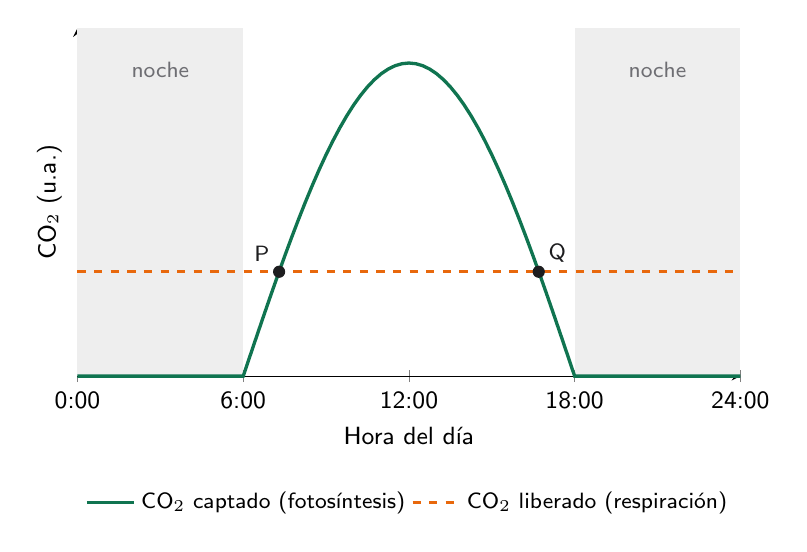
\begin{tikzpicture}[font=\small]
\begin{axis}[width=10cm,height=6cm,axis lines=left,xmin=0,xmax=24,ymin=0,ymax=10,xtick={0,6,12,18,24},xticklabels={0:00,6:00,12:00,18:00,24:00},ytick=\empty,xlabel={Hora del día},ylabel={CO$_2$ (u.a.)},legend style={draw=none,at={(0.5,-0.3)},anchor=north,font=\footnotesize},legend columns=2,legend cell align=left,clip=false]
\fill[gris!12] (axis cs:0,0) rectangle (axis cs:6,10);
\fill[gris!12] (axis cs:18,0) rectangle (axis cs:24,10);
\addplot[menta!70!black,very thick,domain=0:24,samples=97] {x<6 ? 0 : (x>18 ? 0 : 9*sin(deg(pi*(x-6)/12)))};
\addlegendentry{CO$_2$ captado (fotosíntesis)}
\addplot[nar,very thick,dashed] coordinates {(0,3)(24,3)};
\addlegendentry{CO$_2$ liberado (respiración)}
\fill[tinta] (axis cs:7.3,3) circle (2.2pt) node[anchor=south east,font=\footnotesize] {P};
\fill[tinta] (axis cs:16.7,3) circle (2.2pt) node[anchor=south west,font=\footnotesize] {Q};
\node[font=\footnotesize,text=gris] at (axis cs:3,8.8) {noche};
\node[font=\footnotesize,text=gris] at (axis cs:21,8.8) {noche};
\end{axis}
\end{tikzpicture}
\end{document}
